\documentclass{article} 
\usepackage{amsmath} 
\usepackage{amssymb} 
\usepackage{amsthm} 
\usepackage[margin=0.2in]{geometry} 
\usepackage{hyperref} 
\usepackage{physics} 
\usepackage{tikz} 
\usepackage{mathtools}
\mathtoolsset{showonlyrefs} 
\theoremstyle{definition} 
\newtheorem{theorem}{Theorem}[section] 
\newtheorem{corollary}{Corollary}[theorem] 
\newtheorem{lemma}[theorem]{Lemma} 
\newtheorem{definition}{Definition}[section] 

\author{Connor Duncan}
\date{\today}

\title{notes-09-09-2019}
\begin{document}
\abstract{A single document copy of these notes, as well as a mirror of every note, can be found at \url{connorduncan.xyz/notes}}
\subsubsection{Second Order Energy Correction} \begin{equation} \bra{n^0}\left(H_0\ket{n^2}+H_1\ket{n^1}\right)=\bra{n^0}\left(E_n^{(0)}\ket{n^2}+E_n^{(1)}\ket{n^1}+E_n^{(2)}\ket{n^0}\right) \end{equation} we get \begin{equation} E_n^{0}\bra{n^0}\ket{n^2}+\bra{n^0}H_1\ket{n^1}=E_n^{(0)}\bra{n^0}\ket{n^2}+E_n^{(1)}\bra{n^0}\ket{n^1}+E_n^{(2)}\bra{n^0}\ket{n^0} \end{equation} We have cancellation, and also $E_n^{(1)}\bra{n^0}\ket{n^1}\sim0+\mathcal{O}(\lambda^2)$, so we get \begin{equation} E_n^{(2)}=\bra{n^0}H_1\ket{n^{1}}=\sum_{m\neq n} \frac{ \bra{n^0}H_1\ket{m^{0}}\bra{m^0}H_1\ket{n^0} }{E_n^{(0)}-E_m^{(0)}} = \sum_{m\neq n} \frac{ |\bra{m^0}H_1\ket{n^0}|^2}{E_n^{(0)}-E_m^{(0)}} \end{equation} An interesting property of this is level repulsion. Basically, higher order contributions cause repulsion. \begin{center} 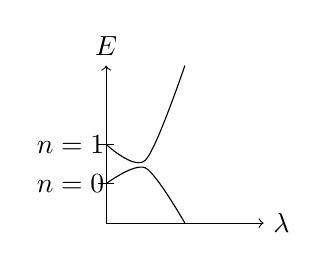
\begin{tikzpicture} \draw[->] (0,0)--(0,2) node[anchor=south] {$E$}; \draw[->] (0,0)--(2,0) node[anchor=west] {$\lambda$}; \foreach \n in {0,1}{ \draw (-.1,{0.5*(\n+1)})--(.1,{0.5*(\n+1)}) node[anchor=east] {$n=\n$}; } \draw plot[smooth] coordinates {(0,0.5) (0.5,0.7) (1,0)}; \draw plot[smooth] coordinates {(0,1) (0.5,0.8) (1,2)}; \end{tikzpicture} \end{center} Take some hamiltonian for the simple harmonic oscillator, however, in the presence of an external electric field. \begin{equation} H=H_0+H_1=\frac{p^2}{2m}+\frac{1}{2}m\omega^2x^2-\mathcal{E}qx \end{equation} \subsubsection{First order} First, we attempt the first order correction \begin{equation} E_n^{(1)}=\bra{n^{(0)}}/H_1\ket{n^{(0)}}=-\mathcal Eq\bra{n^{(0)}}x\ket{n^{(0)}}=0 \end{equation} where the final equality holds by the homework problem where we showed that $x$ can only have non-vanishing matrix elements between states of opposite parity. \subsubsection{Second order} This means we have to go to second order \begin{equation} \ket{n}=\ket{n^{(0)}}-q\mathcal E\sum_{m\neq n}\ket{m^{(0)}}\frac{ \bra{m^{(0}}x\ket{n^{(0)}} }{E_n^{(0)}-E_m^{(0)}} \end{equation} rewriting $x=\sqrt{\frac{\hbar}{2m\omega}}(a+a^\dag)$, we take \begin{align} \ket{n}=\ket{n^{(0)}}-q\mathcal{E}\left(\ket{n^{(0)}+1}\frac{\sqrt{n+1}}{-\hbar\omega}\sqrt{ \frac{\hbar}{2m\omega}}+\ket{n^{(0)}-1}\frac{\sqrt{n}}{\hbar\omega}\sqrt{\frac{\hbar}{2m\omega}}\right) \\ =\ket{n^{(0)}}+\frac{q\mathcal{E}}{\hbar\omega}\sqrt{\frac{\hbar}{2m\omega}} \left(\sqrt{n+1}\ket{n^{(0)}+1}-\sqrt{n}\ket{n^{(0)}-1}\right) \end{align} Then, we calculate the final energy correction as \begin{equation} E_n^{(2)}= \frac{\hbar q^2\mathcal{E}^2}{2m\omega}\left(\frac{n+1}{-\hbar\omega}+\frac{n}{\hbar\omega}\right) = -\frac{q^2\mathcal{E}^2}{2m\omega^2} \end{equation} \subsubsection{Complete the Squares} This is exactly the result that we get from completing the squares and writing \begin{equation} H=\frac{p^2}{2m}+\frac{1}{2}m\omega\left(x-\frac{q\mathcal E}{m\omega^2}\right)^2-\frac{1}{2}\frac{q^2\mathcal{E}^2}{m\omega^2} \end{equation} This gives us exactly the same result, which is a nice sanity check! \subsection{Degenerate Perturbation Theory} If we have some set of degenerate levels, and apply some perturbation, they might split, and be unique \begin{center} 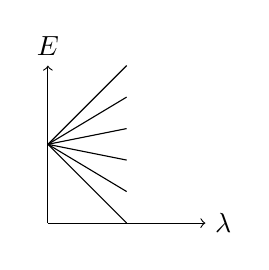
\begin{tikzpicture} \draw[->] (0,0)--(0,2) node[anchor=south] {$E$}; \draw[->] (0,0)--(2,0) node[anchor=west] {$\lambda$}; \foreach \n in {-0.5,-0.3,...,0.5}{ \draw (0,1)--++(1,2*\n); } \end{tikzpicture} \end{center} Basically, we want to diagonalize our perturbation matrix within a basis where the degenerate states are no longer degenerate.
\end{document}
